\documentclass[a4paper, 12pt]{article}%тип документа

%отступы
\usepackage[left=1.5cm,right=1cm,top=2cm,bottom=3cm,bindingoffset=0cm]{geometry}
\setlength{\parindent}{5ex}

%Русский язык
\usepackage[T2A]{fontenc} %кодировка
\usepackage[utf8]{inputenc} %кодировка исходного кода
\usepackage[english,russian]{babel} %локализация и переносы

%Вставка картинок
\usepackage{graphicx}
\graphicspath{{pictures/}}
\DeclareGraphicsExtensions{.pdf,.png,.jpg,}
\usepackage{wrapfig}

%Графики
\usepackage{pgfplots}
\pgfplotsset{compat=1.9}

%Математика
\usepackage{amsmath, amsfonts, amssymb, amsthm, mathtools}

%Таблицы
\usepackage{longtable} 
\usepackage{float}

%Римские цифры
\newcommand{\RomanNumeralCaps}[1]{\uppercase\expandafter{\romannumeral#1}}

\usepackage{multirow}


\begin{document}
	\begin{titlepage}
		\begin{center}
			\textsc{Федеральное государственное автономное образовательное учреждение высшего образования«Московский физико-технический институт (национальный исследовательский университет)»\\[5mm]
			}
			
			\vfill
			
			\textbf{Лабораторная работа: \\[3mm]
				Сверхтонкая структура
				\\[50mm]
			}
			
		\end{center}
		
		\hfill
		\begin{minipage}{.5\textwidth}
			Выполнили студенты:\\[2mm]
			Сериков Василий Романович\\[2mm]
			Группа: Б03-102\\[5mm]
			Сериков Алексей Романович\\[2mm]
			Группа: Б03-102\\[5mm]
			
		\end{minipage}
		\vfill
		\begin{center}
			Москва, 2024 г.
		\end{center}
		
	\end{titlepage}
	
	\newpage
	\textbf{Аннотация}\\
	
	Целью работы является регистрация сверхтонкой структуры спектральных линий, изучение методики работы со сканирующим интерферометром Фабри-Перо.\\
	
	\textbf{Теоретические сведения: }\\
	
	Между различными состояниями электронной оболочки i, k могут происходить оптические переходы, если выполняются правила отбора:
	
	$$ \Delta L = L_i - L_k = \pm 1 $$
	$$ \Delta S = S_i - S_k = 0 $$
	$$ \Delta J = J_i - J_k = 0, \pm 1 \text{    (кроме случая} J_i = J_k) $$
	
	Излучаемая при таких переходах спектральная линия может иметь довольно сложную структуру. Прежде всего следует отметить тонкую структуру спектральных линий, связанную с мультипольностью спектральных термов. В результате взаимодействия между спиновым моментом электронов и моментом их орбитального движения энергия оболочки оказывается зависящей от абсолютного значения вектора полного момента электронной оболочки J. Под влиянием этого взаимодействия вырожденный ранее уровень расщепляется на ряд различных уровней. Каждый терм расщепляется на 2S + 1 (если L > S) или 2L + I (если L < S) состояний. Вследствие этого многие спектральные линии представляют собой дублеты, триплеты и т.д.
	
	Вторым по величине эффектом, влияющим на структуру спектральных линий, является изотопическое смещение. Большинство химических элементов встречаются в виде нескольких изотопов. Электронные оболочки атомов изотопов одного и того же элемента идентичны по числу электронов. Из-за того, что состав ядер изотопов несколько различается, спектральные термы различаются по энергии, следовательно сдвигаются и длины волн спектральных линий.
	
	Также в спектрах проявляется и сверхтонкая структура, обусловленная взаимодействием электронной оболочки с ядром. Атомное ядро обладает собственным механическим моментом I
	
	c которым всегда связан магнитный момент $\vec{\mu}$, определяемый соотношением
	$$
	 \vec{\mu}=\frac{1}{2 c}\left(\frac{l}{m_p}\right) r \vec{I} \text {, }
	$$
	
	где $\frac{e}{m_p}$ - отношение заряда протона к его массе $m_p ; \gamma$ - гиромагнитное соотношение
	$$
	\mu_{\text{яд}}=\frac{h}{4 \pi c}\left(\frac{e}{m_p}\right) 
	$$
	
	Эта величина в 1836 раз меньше магнетона Бора
	$$
	\mu_0=\frac{h}{4 \pi c}\left(\frac{e}{m_e}\right)
	$$
	
	где $m_e$ - масса электрона. Абсолютная величина собственного момента ядра $|\vec{I}|$ связная с квантовым числом $I$ соотношением
	$$
	|\vec{I}|=\frac{h}{2 \pi} \sqrt{I(I+1)}
	$$
	
	
	Максимальное абсолютное значение проекции магнитного ядра на направление внешнего поля, принимаемое обычно за значение магнитного момента ядра, равно
	$$
	\mu=\mu_{\text{яд}} \gamma I \mu
	$$
	
	Полный момент атома $\vec{F}$ равен сумме ядерного момента $\vec{I}$ и момента электронной оболочки J
	$$
	\vec{F}=\vec{I}+\vec{J} 
	$$
	
	Абсолютная величина вектора $\vec{F}$ равна
	$$
	|\vec{F}|=\frac{h}{2 \pi} \sqrt{F(F+1)},
	$$
	
	\textbf{Экспериментальная установка: }\\
	
	Для исследования сверхтонкой структуры линии излучения используется спектрометрическая установка с интерферометром Фабри-Перо, призменным спектрографом ИСП-51, у которого в фокальной плоскости камерного объектива установлена входная щель, и фотоприемника с системой усиления и регистрации сигнала.
	
	\begin{figure}[H]
		\centering
		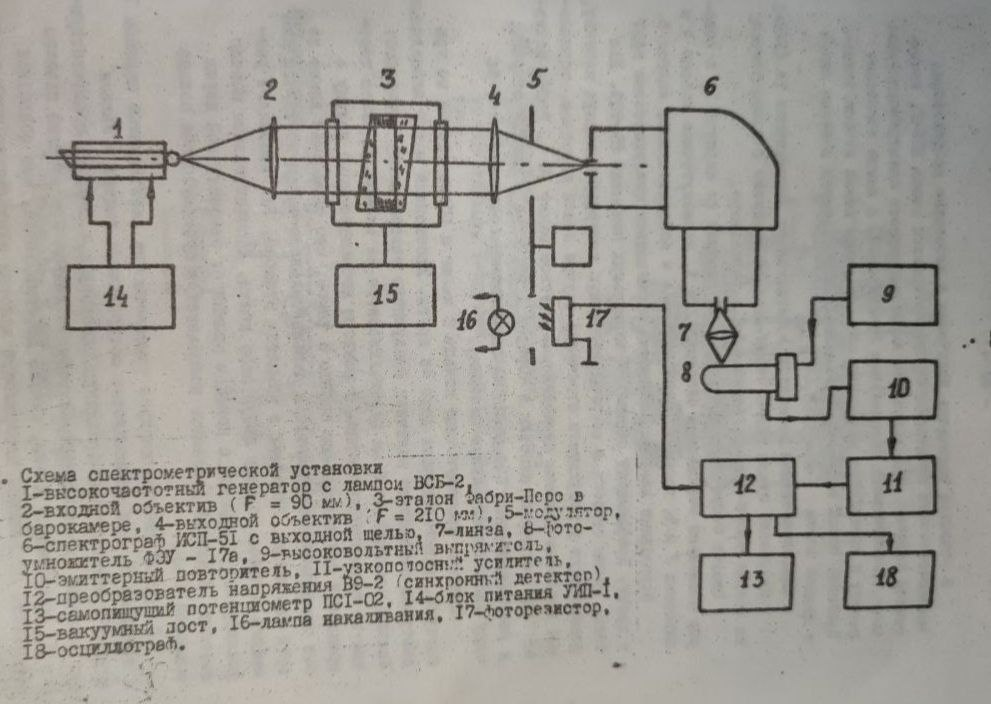
\includegraphics[width=1\linewidth]{ust.jpeg}
		\caption{Экспериментальная установка}
	\end{figure}
		\begin{figure}[H]
		\centering
		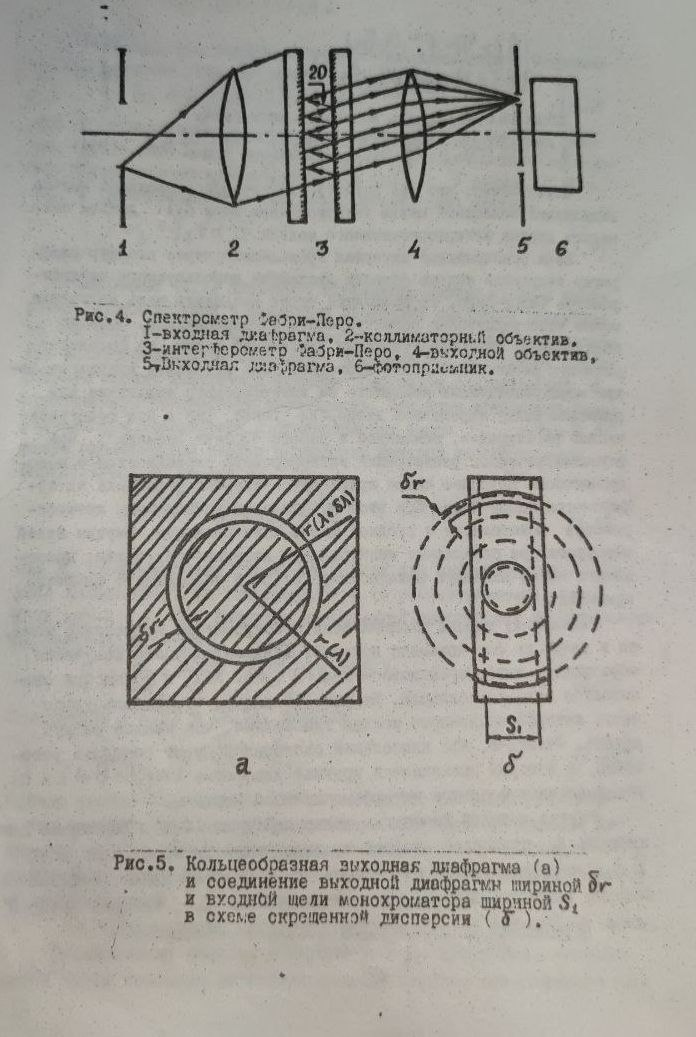
\includegraphics[width=1\linewidth]{F-P.jpg}
	\end{figure}
	\begin{figure}[H]
		\centering
		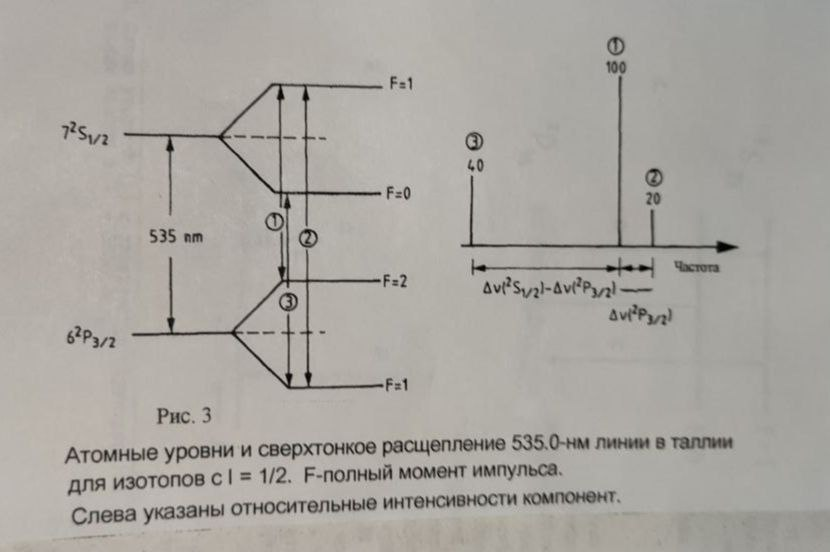
\includegraphics[width=1\linewidth]{levels.jpeg}
	\end{figure}
	

	\newpage
	
	\textbf{Ход работы: }\\
	\begin{enumerate}
	\item Для регистрации сверхтонкого расщепления мы откачали воздух из барокамеры с помощью форвакуумного насоса и наблюдали изменение интерференционной картины. На экране монитора получили следующую картину:
	
	

	\begin{figure}[H]
	\centering
	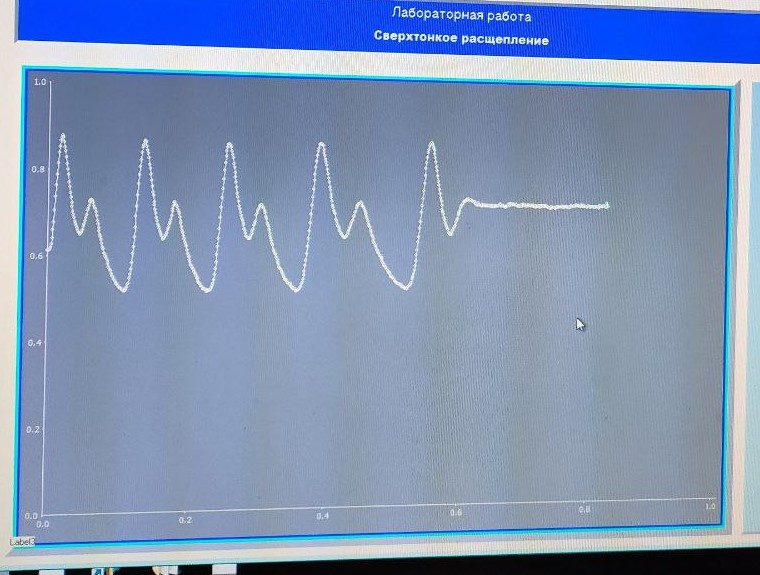
\includegraphics[width=0.8\linewidth]{result.jpg}
	\caption{Результат обработки данных с детектора при отсутствии диафрагмы Гартмана}
	\end{figure}
	
 	\begin{figure}[H]
		\centering
		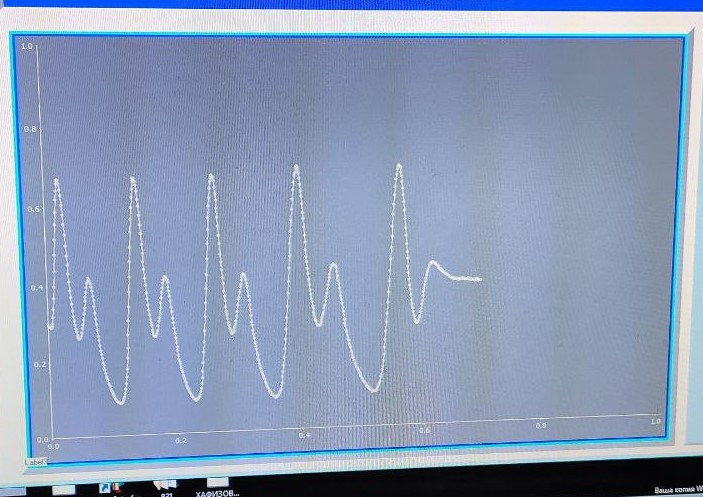
\includegraphics[width=0.8\linewidth]{result_1.jpg}
		\caption{Результат обработки данных с детектора при наличии диафрагмы Гартмана}
	\end{figure}
	
	\item Проведем расчет расщепления по следующим формулам: 
	$$ m_0 = 2d/\lambda_0 \cdot n $$
	$$ \phi_h=\arcsin \left[n \sqrt{\left(1-\left(\frac{m}{m_0}\right)^2\right)}\right] = 0,02690 \text{рад}$$
	
	$$ \phi_1=\arcsin \left(n\sqrt{\left(1-\left(\frac{m}{m_0}\left(1+\frac{\Delta \lambda}{\lambda_0}\right)\right)^2\right)} \right). = 0,02400 \text{рад}$$ 
	
	$$ \delta \lambda=\lambda\left(\frac{m_0}{m}-1\right) \sqrt{1-\frac{1}{n^2} \sin \left(\phi_{\text {mid }}\right)} = 0,06 \text{\AA} $$

 	$$\Delta m = \frac{2}{d}(n_0 - 1)\frac{\Delta P}{P_0}$$
	\end{enumerate}
	 	

	\begin{longtable}{|c|c|c|c|c|c|}
 		\hline
 		$P_0$, атм & 1 & 0,8 & 0,6 & 0,4 & 0,2  \\ \hline
 		$\Delta m$	& 0,21 & 0,27 & 0,36 & 0,54 & 1,09  \\ \hline
 		$ \delta \lambda $, \AA & 0,4987 & 0,4986 & 0,4984 & 0,4979 & 0,4972 \\ \hline
 		\caption{Полученные результаты}
 	\end{longtable}

	\textbf{Результаты: }\\
	
	В ходе работы мы изучили устройство интерферометра фабри-Перо и получили спектр сверхтонкого расщепления линий Tl с $\lambda$ = 5350,46 \AA. Полученное значение расщепления $\delta \lambda \approx 0,5$ \AA  совпадает по порядку со значением из методички равным $\delta \lambda \approx 0,1$ \AA
	\end{document}